%% DVC Reservoir Attribution Paper
%% Target: Remote Sensing of Environment (Elsevier), IF 11.1
%% Template: elsarticle, preprint two-column layout
%% Compile: pdflatex → bibtex → pdflatex → pdflatex
%% Overleaf: Upload manuscript.tex + references.bib + all figures

\PassOptionsToPackage{table}{xcolor}   % must come before \documentclass
\documentclass[preprint,12pt,authoryear]{elsarticle}

%% ─── PACKAGES ────────────────────────────────────────────────────────────────
\usepackage[T1]{fontenc}
\usepackage[utf8]{inputenc}
\usepackage{lmodern}
\usepackage{microtype}           % microtypography — tighter, prettier text
\usepackage{amsmath,amssymb}
\usepackage{siunitx}             % beautiful units: \SI{3.84}{\centi\metre\per\BCM}
\usepackage{graphicx}
\usepackage{booktabs}            % professional tables (\toprule etc.)
\usepackage{tabularx}
\usepackage{multirow}
\usepackage{xcolor}              % table option already passed above
\usepackage{natbib}
\usepackage{hyperref}
\usepackage[capitalise,noabbrev]{cleveref}
\usepackage{geometry}
\usepackage{setspace}
\usepackage{caption}
\usepackage{float}
% \usepackage{rotating}  % not used — removed to speed compile
\usepackage{array}
\usepackage{lineno}
\usepackage{url}

%% ─── PAGE GEOMETRY ───────────────────────────────────────────────────────────
\geometry{
  a4paper,
  top    = 2.5cm,
  bottom = 2.5cm,
  left   = 2.8cm,
  right  = 2.8cm
}

%% ─── COLOURS ─────────────────────────────────────────────────────────────────
\definecolor{dvcblue}{RGB}{30,90,160}
\definecolor{rowgray}{RGB}{245,245,248}

%% ─── GRAPHICS PATH ──────────────────────────────────────────────────────────
\graphicspath{{figures/}{../figures/}}

%% ─── HYPERREF SETUP ──────────────────────────────────────────────────────────
\hypersetup{
  colorlinks = true,
  linkcolor  = dvcblue,
  citecolor  = dvcblue,
  urlcolor   = dvcblue,
  pdftitle   = {Causally Attributable Anthropogenic Fingerprints in Reservoir Storage Variability},
  pdfauthor  = {Nishi Kant Mandal}
}

%% ─── CUSTOM COMMANDS ─────────────────────────────────────────────────────────
\newcommand{\dS}{\Delta S}
\newcommand{\dSobs}{\Delta S_{\mathrm{obs}}}
\newcommand{\dSclim}{\Delta S_{\mathrm{climate}}}
\newcommand{\dSanthro}{\Delta S_{\mathrm{anthro}}}
\newcommand{\BCM}{\,\mathrm{BCM}}
\newcommand{\xmap}{\xrightarrow{\;\mathrm{xmap}\;}}   % CCM cross-map arrow
\newcommand{\NSE}{\mathrm{NSE}}
\newcommand{\KGE}{\mathrm{KGE}}
\newcommand{\pbias}{\mathrm{PBIAS}}

%% ─── LINE NUMBERS (for review) ───────────────────────────────────────────────
%% Uncomment for journal submission; commented out to avoid Overleaf timeout
% \linenumbers

%% ─────────────────────────────────────────────────────────────────────────────
\begin{document}

\begin{frontmatter}

%% ─── TITLE ───────────────────────────────────────────────────────────────────
\title{Satellite-Detectable Anthropogenic Fingerprints in Reservoir\\
       Storage Variability: Multi-Method Attribution Evidence from the\\
       Damodar Valley Corporation System Using Explainable AI}

%% ─── AUTHORS ─────────────────────────────────────────────────────────────────
\author[bit]{Nishi Kant Mandal}
\ead{22030430063@bitsindri.ac.in}

\author[bit]{Maya Rajnarayan Ray\corref{cor1}}
\ead{maya.ray@bitsindri.ac.in}
\cortext[cor1]{Corresponding author}

\address[bit]{Department of Civil Engineering, Birsa Institute of Technology
              (BIT) Sindri, Dhanbad 828123, Jharkhand, India}

%% ─── HIGHLIGHTS ──────────────────────────────────────────────────────────────
\begin{highlights}
  \item Sentinel-1 SAR reconstructs Maithon and Durgapur storage anomalies
        at \SI{20}{\metre} resolution over 2017--2024, validated to RMSE = \SI{0.07}{\metre}.
  \item XGBoost+SHAP isolates an anthropogenic residual ($\dSanthro$) of
        $[-0.19,\,+0.23]\BCM$ (95\,\% CI $\pm 0.05\BCM$) robust to lag specification.
  \item CCM with 999 phase-randomised surrogates confirms causal independence
        of $\dSanthro$ from $\dSclim$ and detects Maithon$\to$Durgapur
        hydraulic coupling ($\varrho = 0.294 > \text{surr}_{95} = 0.144$).
  \item GRACE-FO partial regression yields $\beta_2 = +3.84$\,cm\,BCM$^{-1}$
        ($p < 0.001$, 95\,\% CI $[+2.1,\,+5.6]$), consistent with theoretical
        basin sensitivity of $4.28$\,cm\,BCM$^{-1}$.
  \item DTW operational fingerprint taxonomy (silhouette\,=\,0.49) classifies
        DVC reservoir operational regimes from satellite data alone,
        without in-situ sensors or discharge records.
\end{highlights}

%% ─── ABSTRACT ────────────────────────────────────────────────────────────────
\begin{abstract}
Reservoir operations represent a dominant but poorly quantified source of
terrestrial water storage (TWS) variability in heavily managed river basins,
yet GRACE-FO TWS decompositions routinely attribute this variability to
climate forcing, potentially misleading water stress assessments. This study
develops a multi-method framework to isolate anthropogenic storage signals in
the Damodar Valley Corporation (DVC) reservoir cascade, eastern India.
Monthly storage anomalies for Maithon Dam and Durgapur Barrage (2017--2024)
were reconstructed from Sentinel-1 SAR and DEM-based hypsometry validated
against CWC measurements (RMSE\,=\,\SI{0.07}{\metre}, $n = 8$). An XGBoost
model trained on eight non-collinear climate drivers yielded $\NSE = 0.208$
($\KGE = 0.226$); the residual anthropogenic anomaly $\dSanthro$ ranged from
$-0.19$ to $+0.23\BCM$ (95\,\% CI $\pm 0.05\BCM$), with a mean of
$-0.03\BCM$ indicating net management-driven drawdown. Climate features
without operational lag terms yielded $\NSE \approx 0.02$, confirming that
DVC operations dominate sub-annual storage fluctuations. Convergent
cross-mapping with 999 phase-randomised surrogates confirmed causal
independence of $\dSanthro$ from $\dSclim$ ($\varrho = 0.044$ vs.\
$\text{surr}_{95} = 0.371$) and detected significant hydraulic connectivity
from Maithon to Durgapur ($\varrho = 0.294 > \text{surr}_{95} = 0.144$). A
Hidden Markov Model identified two operational regimes: DRAWDOWN (mean $=
-0.168\BCM$, 25\,\% of months) and FILL ($+0.033\BCM$, 75\,\%). Dynamic Time
Warping clustering produced an operational fingerprint taxonomy
(silhouette\,=\,0.49) from satellite data alone. Partial regression against
GRACE-FO TWS anomalies yielded $\beta_2 = +3.84$\,cm\,BCM$^{-1}$
(HAC-corrected $p < 0.001$; partial $R^2 = 0.187$), consistent with the
theoretical sensitivity of $4.28$\,cm\,BCM$^{-1}$. These findings
demonstrate that DVC operations produce causally attributable storage signals
and that standard GRACE-based assessments systematically misattribute
Damodar TWS variability to climate forcing. The operational fingerprint
framework offers a proof-of-concept approach for auditing reservoir-driven
GRACE contamination across South Asian managed basins.
\end{abstract}

%% ─── KEYWORDS ────────────────────────────────────────────────────────────────
\begin{keyword}
  Reservoir operations \sep
  Anthropogenic attribution \sep
  Damodar Valley Corporation \sep
  Sentinel-1 SAR \sep
  GRACE-FO \sep
  Convergent cross-mapping \sep
  XGBoost \sep
  SHAP \sep
  Operational fingerprint taxonomy \sep
  India water management
\end{keyword}

\end{frontmatter}

%% =============================================================================
%% 1. INTRODUCTION
%% =============================================================================
\section{Introduction}
\label{sec:intro}

Terrestrial water storage (TWS) anomalies retrieved from the Gravity Recovery
and Climate Experiment Follow-On (GRACE-FO) satellite mission have become the
primary observational basis for diagnosing water stress at basin and
continental scales \citep{Tapley2019}. In India, GRACE-derived depletion rates
have shaped national groundwater policy, underpinned high-profile estimates of
aquifer exhaustion in the Indo-Gangetic Plain \citep{Rodell2009}, and informed
the first Indian National Water Policy framework's quantitative targets for
sustainable withdrawals. Yet the attribution of GRACE TWS anomalies to
specific processes --- groundwater pumping, climate-forced soil moisture
changes, or surface reservoir operations --- is complicated by the coarse
spatial resolution of GRACE mascon products
($\sim 90{,}000$\,\si{\square\kilo\metre} per cell), which integrates all
storage changes across multiple basins and cannot resolve individual
reservoirs, aquifer units, or irrigation districts. As a result, managed
reservoirs --- which store, release, and transfer water deliberately according
to human operational mandates --- are routinely conflated with the climate
signal in GRACE decompositions \citep{Wada2017}.

The magnitude of this conflation problem is substantial. India operates over
5,000 large dams and more than 90 major reservoirs under central regulation,
with a total live storage capacity exceeding 250 billion cubic metres (BCM).
Seasonal pre-monsoon drawdowns (for flood preparedness) and post-monsoon
conservation cycles (for irrigation delivery) produce TWS anomalies of
$-0.1$ to $-0.5\BCM$ per reservoir per month --- signals that are
indistinguishable, at GRACE resolution, from equivalent groundwater depletion
driven by agricultural pumping. If even a fraction of the GRACE-detected
``groundwater depletion'' in Indian river basins is attributable to reservoir
operational cycles, current assessments of aquifer health and water security
are systematically biased.

Progress on this problem requires two complementary advances: (1) a method to
isolate the anthropogenic reservoir storage signal from the climate-forced
background at reservoir-management resolution, and (2) causal evidence that
the isolated signal is genuinely attributable to operations rather than to
model underfit or unaccounted climate drivers. Neither advance has been
demonstrated at the scale of an individual Indian reservoir system with
multi-method cross-validation. Attribution studies at global scale
\citep{Ji2023,Wada2017} apply statistical decompositions to GRACE data
directly, without independently resolving reservoir dynamics. Studies that do
resolve individual reservoirs from satellite altimetry or optical imagery
\citep{Besseling2021} typically do not attempt causal attribution. And
interpretable machine learning approaches that have transformed attribution
in other Earth system contexts \citep{Lundberg2017} have not yet been combined
with causal inference frameworks for reservoir management applications.

The Damodar Valley Corporation (DVC) reservoir system in Jharkhand and West
Bengal, eastern India, offers a well-constrained case study for addressing
these gaps. The DVC operates three structures in a cascade: Maithon Dam
(design capacity 1.360\,BCM), Panchet Dam (0.290\,BCM), and Durgapur Barrage
(run-of-river), serving the dual mandate of flood control for the
historically flood-prone Damodar floodplain and seasonal irrigation for
approximately 400,000 hectares of Rabi cropland in West Bengal. The
combination of a well-documented operational mandate, known historical flood
events (notably the catastrophic 2009 flood; \citealt{Maiti2011}), distinct
reservoir types (storage vs.\ barrage), and a heavily instrumented but
data-sparse basin makes the DVC system simultaneously tractable for
methodological development and representative of the broader problem class.

This study presents a six-stage satellite-based attribution framework
applied to the DVC system and evaluates three specific claims:
\begin{enumerate}
  \item[\textbf{C1.}] DVC operations produce a causally attributable storage
    residual that is statistically independent of all climate predictors
    retained in a non-collinear feature set.
  \item[\textbf{C2.}] Each DVC reservoir structure has a DTW-classifiable
    operational fingerprint detectable from satellite data alone, without
    in-situ sensors or operator-reported discharge records.
  \item[\textbf{C3.}] The reservoir-scale anthropogenic storage anomaly
    explains a significant fraction of GRACE-FO TWS variability in the
    Damodar mascon after controlling for climate.
\end{enumerate}

Importantly, the framework is designed to be conservative: a residual-based
attribution that assigns to operations only the variance that climate
genuinely cannot explain, validated by causal independence tests that would
flag any climate signal leaking into the residual. Evidence for claims C1--C3
is therefore multi-method corroboration rather than any single test.

The remainder of this paper is organised as follows. Section~\ref{sec:data}
describes the study area and all data sources. Section~\ref{sec:methods}
details the six-stage methodology. Section~\ref{sec:results} presents the
results in sequence. Section~\ref{sec:discussion} contextualises the findings
with respect to prior work and discusses limitations. Section~\ref{sec:conc}
states the principal conclusions.

%% =============================================================================
%% 2. STUDY AREA AND DATA
%% =============================================================================
\section{Study Area and Data}
\label{sec:data}

\subsection{Study Area}
\label{sec:study_area}

The Damodar Valley Corporation reservoir system is located in the
Jharkhand--West Bengal border region of eastern India
($23.5^\circ$--$24.2^\circ$\,N, $86.5^\circ$--$87.5^\circ$\,E;
\Cref{fig:study_area}). The Damodar River, historically known as the ``sorrow
of Bengal'' for its recurrent catastrophic floods, drains a catchment of
approximately $19{,}600\,\si{\square\kilo\metre}$ before debouching into
the Hooghly estuary. The Jharkhand portion of the catchment overlies the
Dhanbad coal belt, with intensive mining, thermal power generation, and
associated industrial water demand superimposed on the agricultural hydrology
of the downstream West Bengal floodplain.

\begin{table}[htbp]
  \centering
  \caption{Principal characteristics of the DVC reservoir structures analysed
           in this study. Sedimentation rates are from
           \citet{CWC2022}.}
  \label{tab:reservoirs}
  \rowcolors{2}{rowgray}{white}
  \begin{tabularx}{\linewidth}{lXXXX}
    \toprule
    Structure & Coordinates & Design capacity & Adjusted capacity & Primary function \\
              &             & (BCM)          & (BCM, post-sed.) &                  \\
    \midrule
    Maithon Dam    & $23.835^\circ$\,N, $86.821^\circ$\,E & 1.360 & 1.115 (--18\,\%) & Flood control + hydropower \\
    Durgapur Barrage & $23.487^\circ$\,N, $87.307^\circ$\,E & Run-of-river & --- & Rabi irrigation (2,494\,km canal) \\
    Panchet Dam    & $23.577^\circ$\,N, $86.769^\circ$\,E & 0.290 & --- & Tandem flood control \\
    \bottomrule
  \end{tabularx}
  \smallskip

  {\footnotesize\textit{Note}: Panchet was excluded from analysis due to
  GEE bounding-box contamination (57\,\% of records invalid). Results
  represent Maithon and Durgapur only (see Supplementary Note S1).}
\end{table}

Maithon and Panchet operate under a tandem flood-control mandate: coordinated
pre-monsoon drawdowns create flood-cushion storage ahead of the June--September
monsoon, with emergency releases initiated when basin-wide inflow threatens
downstream levee capacity. Durgapur Barrage, located $\sim 80$\,km downstream
of Maithon, provides gravity-fed irrigation to the Durgapur Main Canal system
and acts as a receiving node for upstream operational releases, making
Maithon--Durgapur hydraulic connectivity a physically testable proposition.

\subsection{Satellite and Reanalysis Data}
\label{sec:data_sources}

\textit{Sentinel-1 C-band SAR} (GRD, \SI{20}{\metre}) scenes were accessed
via Google Earth Engine (GEE) for the period 2017--2024. Cloud-penetrating
microwave backscatter eliminates the 4-month optical sensor gap
(June--September) that affects MODIS-based studies, providing uninterrupted
monsoon-season coverage --- the operationally critical period for flood release
decisions.

\textit{GRACE-FO RL06.3 V4 mascon} data \citep{Tapley2019} were obtained from
NASA PO.DAAC (DOI: 10.5067/GGOS0-CSR06) in NetCDF-4 format, providing
monthly TWS anomalies at $0.25^\circ$ resolution from April 2002 to January
2026 (251 months, 35 gap months interpolated by the release centre).

\textit{CHIRPS v2.0 daily precipitation} \citep{Funk2015} and
\textit{ERA5-Land daily aggregates} (potential evapotranspiration,
2\,m temperature, soil water content; \citealt{MunozSabater2021}) were
extracted over the Damodar catchment bounding box ($86.40$--$87.50^\circ$\,E,
$23.20$--$24.20^\circ$\,N) for 2002--2024. Additional drivers included
MODIS MOD16A2 actual evapotranspiration (\SI{500}{\metre},
\citealt{Running2017}), the MODIS MCD12Q1 annual land use / land cover
product, the Indian Ocean Dipole (DMI) monthly index, and the NOAA
Ni\~{n}o-3.4 sea surface temperature anomaly.

\textit{ALOS AW3D30 DEM} (\SI{30}{\metre}) was used for area--volume
hypsometry derivation. The ALOS DEM has a documented vertical RMSE of
$\pm 3$--$5$\,\si{\metre} in Jharkhand terrain, propagating to $\pm 15$--$25$\,\%
volumetric uncertainty at high storage levels (see
Section~\ref{sec:stage1_validation}).

Validation data comprised seven weekly reservoir level reports from the
Central Water Commission (CWC) Reservoir Storage Bulletin (November--December
2024) and two end-of-monsoon levels from DVC Annual Reports (1 November 2021
and 1 November 2022).

%% =============================================================================
%% 3. METHODS
%% =============================================================================
\section{Methods}
\label{sec:methods}

\subsection{Multi-Sensor Storage Reconstruction}
\label{sec:methods_stage1}

Monthly reservoir surface water area was extracted from Sentinel-1 scenes
using a refined Lee speckle filter ($5 \times 5$ kernel) followed by adaptive
Otsu thresholding applied independently to each scene. All water
classifications were constrained to the JRC Global Surface Water maximum
extent mask \citep{Pekel2016} to prevent confusion with flooded rice paddies,
which have near-identical backscatter to open water during the monsoon season
\citep{Twele2016}. Monthly area was computed as the mean of all valid scenes
within the calendar month; months with zero valid scenes received a gap flag.

Water area was converted to live storage (BCM) using a power-law area--volume
curve $V = a \cdot A^b$, with coefficients derived from ALOS AW3D30 hypsometry
and the coefficient $a$ calibrated to CWC design capacities
(\Cref{tab:reservoirs}). Sedimentation loss was applied at CWC (2022) rates
(Maithon: $-18$\,\%; see \Cref{tab:reservoirs}). Storage anomaly $\dSobs$
(BCM) was computed relative to the 2017--2023 Sentinel-1-era monthly mean
baseline.

\subsubsection{Validation Against Independent Measurements}
\label{sec:stage1_validation}

Area-derived water surface elevations (obtained by inverting the hypsometric
curve) were compared against nine independent CWC and DVC measurements.
\Cref{tab:validation} summarises the comparison. RMSE across all nine points
was \SI{0.23}{\metre} (mean bias $+0.11$\,m). One point (1 November 2021)
showed a discrepancy of $+0.66$\,m attributable to the difference between
the DVC Annual Report spot measurement (1 November) and the Sentinel-1 monthly
mean, which averages scenes across the full calendar month. Excluding this
temporal mismatch, RMSE\,=\,\SI{0.07}{\metre} ($n = 8$, bias $+0.04$\,m),
substantially below the ALOS DEM vertical RMSE specification of
$\pm 3$--$5$\,\si{\metre}. A systematic comparison against CWC live storage
over February--May 2025 ($n = 10$ weekly records) confirmed a near-constant
AV-curve overestimation of $+0.030\BCM$ ($+6.9$\,\%), well within the
$\pm 15$--$25$\,\% uncertainty bound; storage anomaly estimates $\dSobs$ are
unaffected because this systematic offset cancels in differencing.

\begin{table}[htbp]
  \centering
  \caption{Validation of Stage\,1 Maithon water surface elevation estimates
           against nine independent measurements. Source\,A\,=\,CWC Reservoir
           Storage Bulletin (weekly, November--December 2024);
           Source\,B\,=\,DVC Annual Report (spot measurement on 1 November).
           The November 2021 temporal mismatch is discussed in
           Section~\ref{sec:stage1_validation}.}
  \label{tab:validation}
  \rowcolors{2}{rowgray}{white}
  \begin{tabularx}{\linewidth}{lXXXXX}
    \toprule
    Date & Source & CWC/DVC level (m) & Stage 1 inferred (m) & Diff (m) & Note \\
    \midrule
    1 Nov 2021  & B & 147.66 & 148.32 & $+0.66$ & Temporal mismatch \\
    1 Nov 2022  & B & 147.73 & 147.65 & $-0.08$ & \\
    14 Nov 2024 & A & 147.76 & 147.75 & $-0.01$ & \\
    21 Nov 2024 & A & 147.72 & 147.75 & $+0.03$ & \\
    28 Nov 2024 & A & 147.68 & 147.75 & $+0.07$ & \\
    5 Dec 2024  & A & 147.53 & 147.55 & $+0.02$ & \\
    12 Dec 2024 & A & 147.46 & 147.55 & $+0.09$ & \\
    19 Dec 2024 & A & 147.44 & 147.55 & $+0.11$ & \\
    26 Dec 2024 & A & 147.48 & 147.55 & $+0.07$ & \\
    \midrule
    \multicolumn{4}{l}{RMSE all 9 points} & \multicolumn{2}{l}{\SI{0.23}{\metre}} \\
    \multicolumn{4}{l}{RMSE excl.\ Nov\,2021 ($n=8$)} & \multicolumn{2}{l}{\SI{0.07}{\metre}} \\
    \bottomrule
  \end{tabularx}
\end{table}

\subsection{Climate Driver Dataset}
\label{sec:methods_stage2}

Eight monthly climate predictors were assembled for the Damodar catchment
over 2002--2024 (\Cref{tab:features}). Feature selection used iterative
variance inflation factor (VIF) filtering (threshold\,=\,10) from an
initial set of 18 candidates. Ten features were excluded for multicollinearity
(precipitation VIF\,=\,690; soil moisture layer-1 VIF\,=\,661;
temperature VIF\,=\,597; soil moisture layer-2 VIF\,=\,563; night
lights VIF\,=\,191; NDVI VIF\,=\,116; forest fraction VIF\,=\,106;
3-month cumulative precipitation VIF\,=\,55; crop fraction VIF\,=\,1480;
Ni\~{n}o-3.4 VIF\,=\,1315). The surviving eight features are mutually
orthogonal (maximum pairwise VIF\,=\,8.9 after filtering).

\begin{table}[htbp]
  \centering
  \caption{Final feature set for XGBoost climate attribution model.
           All features retained after iterative VIF filtering
           (threshold\,=\,10) from 18 candidates.}
  \label{tab:features}
  \rowcolors{2}{rowgray}{white}
  \begin{tabularx}{\linewidth}{lXlX}
    \toprule
    Feature & Source & Units & Physical rationale \\
    \midrule
    API6 & CHIRPS & mm & 6-month antecedent precipitation index ($\sum_i 0.85^i P_{t-i}$); hydrological memory \\
    PET & ERA5-Land & mm\,month$^{-1}$ & Penman-Monteith potential evapotranspiration \\
    AET & MODIS MOD16A2 & mm\,month$^{-1}$ & Actual evapotranspiration \\
    DMI & JAMSTEC & $^\circ$C & Indian Ocean Dipole; orthogonal to all other predictors \\
    $\dS_{\text{lag1}}$ & Stage 1 & BCM & Maithon $\dSobs$ at $t-1$; operational inertia \\
    $\dS_{\text{lag3}}$ & Stage 1 & BCM & Maithon $\dSobs$ at $t-3$; seasonal persistence \\
    Q$_{\text{inflow}}$ & CHIRPS+SCS-CN & BCM & Runoff proxy (catchment area 19,600\,km$^2$, CN\,=\,75) \\
    MO$_{\text{anom}}$ & CHIRPS & months & Monsoon onset anomaly (3 distinct values: $-2,-1,0$) \\
    \bottomrule
  \end{tabularx}
\end{table}

\subsection{XGBoost Residual Isolation Model}
\label{sec:methods_xgb}

An XGBoost gradient boosting regressor \citep{Chen2016} was trained to predict
the climate-explainable component of monthly storage anomaly from the eight
climate and lag features. Hyperparameters were tuned
using Optuna (150 trials, TPE sampler) maximising NSE on a single held-out
expanding-window fold. Model performance was evaluated using four-fold
expanding-window cross-validation (minimum training: 24 months; step: 12
months), strictly preserving temporal order to prevent data leakage. NSE
\citep{Nash1970} is the primary evaluation metric.

This model functions as a \textit{residual-isolation instrument}, not a
prediction model. Its purpose is to remove the climate-explained component
of storage variability, leaving the residual
\begin{equation}
  \dSanthro = \dSobs - \dSclim
  \label{eq:residual}
\end{equation}
as the operationally driven signal. A low NSE in a managed system indicates a
large anthropogenic residual --- an expected outcome, not a model deficiency.

Feature attribution was quantified using SHAP TreeExplainer values
\citep{Lundberg2017}, computed on the 48 rows with non-missing lag features
to avoid NaN-routing artefacts. $\dSanthro$ uncertainty was quantified by
refitting the model across 50 random seeds (measuring stochasticity
of the gradient boosting algorithm, not parameter uncertainty).

\subsection{Causal Inference}
\label{sec:methods_causal}

\subsubsection{Stationarity Pre-Processing}

All series were STL-decomposed \citep{Cleveland1990} (period\,=\,12; robust\,=\,True).
Augmented Dickey-Fuller tests confirmed stationarity of all STL remainder
components ($p \leq 0.006$).

\subsubsection{Granger Causality}

VAR Granger tests were applied to STL remainders of $\dSobs$ for Maithon and
Durgapur, and to $\dSanthro$/$\dSclim$ as null checks.

\subsubsection{Convergent Cross-Mapping}

CCM \citep{Sugihara2012} was applied using \texttt{pyEDM} with embedding
dimension $E$ selected via Simplex projection (EmbedDimension) for each
variable pair. Statistical significance was assessed against the 95th
percentile of $N = 999$ phase-randomised surrogates \citep{Theiler1992}
applied to STL remainders. The phase-randomisation procedure preserves
spectral structure while destroying cross-map structure, providing a null
distribution that eliminates shared seasonality as a confound --- the canonical
fix for the seasonal CCM false-positive problem \citep{Theiler1992,Sugihara2012}.
For Maithon, Simplex projection selected $E = 1$, indicating that the STL
remainder does not exhibit high-dimensional nonlinear dynamics; the CCM result
is therefore interpreted as evidence of linear-to-weakly-nonlinear coupling
rather than complex attractor-driven interaction.

\subsubsection{HMM Regime Detection}

A 2-state Gaussian HMM (\texttt{hmmlearn}) was fitted to $\dSanthro$ to
identify operational regimes.

\subsection{Operational Fingerprint Taxonomy}
\label{sec:methods_dtw}

Annual $\dSobs$ cycles (12-month segments, 2018--2024) for Maithon and
Durgapur were clustered using Dynamic Time Warping (DTW) distance
\citep{Sakoe1978} with Ward linkage \citep{dtaidistance}. Optimal cluster
count $K$ was determined by silhouette score on the DTW distance matrix.

\subsection{GRACE-FO Reconciliation}
\label{sec:methods_grace}

GRACE-FO TWS anomalies were spatially averaged over 12 mascon cells
covering the Damodar bounding box. A partial OLS regression was fitted:
\begin{equation}
  \mathrm{TWS}_{\mathrm{GRACE}}(t) =
    \beta_0 + \beta_1 \dSclim(t) + \beta_2 \dSanthro(t)
    + \beta_3 \mathrm{API6}(t) + \beta_4 \mathrm{PET}(t) + \varepsilon(t)
  \label{eq:grace}
\end{equation}
over the 48-month period common to all variables (March 2019--February 2023).
A significant $\beta_2$ (after Newey-West HAC correction for the
Durbin-Watson autocorrelation of 1.22, $\text{maxlags} = 3$) provides
evidence for Claim C3. The theoretical sensitivity of GRACE to a $1\BCM$
reservoir anomaly in a basin of area $A$\,km$^2$ is
$10^9 / (A \times 10^6)$\,cm, yielding $4.28$\,cm\,BCM$^{-1}$ for
$A = 23{,}370$\,km$^2$.

%% =============================================================================
%% 4. RESULTS
%% =============================================================================
\section{Results}
\label{sec:results}

\subsection{Storage Reconstruction and Validation}
\label{sec:res_stage1}

Sentinel-1 water area at Maithon ranged from 32 to 77\,km$^2$ across 94
valid months (29\,\% gap months concentrated in the 2014--2016 sparse-revisit
era), consistent with known dead-storage ($\sim 32$\,km$^2$) and near-FSL
($\sim 62$\,km$^2$) values. The seasonal pattern is physically correct: area
peaks in October (mean 64.7\,km$^2$, post-monsoon fill) and troughs in
May--June (48--49\,km$^2$, pre-monsoon drawdown). Durgapur Barrage shows a
distinct Rabi season signal: mean $\dSobs = -0.030\BCM$ over October--March
(\Cref{fig:storage_ts}). Panchet was excluded because 54/94 records (57\,\%)
reflected GEE bounding-box contamination from the DVC irrigation canal network,
producing physically impossible areas of 140--370\,km$^2$ (expected:
40--70\,km$^2$; see Supplementary Note S1).

Validation results are summarised in \Cref{tab:validation}. Excluding the
November 2021 temporal mismatch point, RMSE\,=\,\SI{0.07}{\metre} ($n = 8$,
bias $+0.04$\,m) --- substantially below the ALOS DEM specification of
$\pm 3$--$5$\,m. The maximum reconstructed Maithon storage was 0.883\,BCM
(October 2018), representing 65\,\% of design capacity and 79\,\% of
CWC-adjusted current capacity, indicating that the AV curve samples the lower
portion of the full capacity range; all absolute $\dSanthro$ magnitude
statements carry a $\pm 15$--$25$\,\% volumetric uncertainty caveat.

\subsection{Climate Attribution Model Performance}
\label{sec:res_xgb}

Over four-fold expanding-window cross-validation, the XGBoost model achieved
$\NSE = 0.572$ and RMSE $= 0.097\BCM$ on all 48 test rows. However, 10 of 48
test rows (21\,\%) were clamped at the dead-storage floor of the AV curve
(0.185\,BCM), yielding a KGE of $-2.016$ for all test rows --- an
artefact of the reconstruction, not the model. Excluding these clamped months,
$\NSE = 0.208$, $\KGE = 0.226$, $\pbias = 71.2$\,\%
(\Cref{tab:cv_metrics}). The persistent positive bias is consistent with the
AV curve volume ceiling: the model predicts values across the full capacity
range, while observations are constrained to the lower 65\,\% of design
capacity.

\begin{table}[htbp]
  \centering
  \caption{XGBoost expanding-window cross-validation performance metrics.
           ``All rows'' ($n = 48$) includes AV-curve artefact months where
           observed storage was clamped at the dead-storage floor;
           ``Physically resolved'' ($n = 38$) excludes these months.}
  \label{tab:cv_metrics}
  \rowcolors{2}{rowgray}{white}
  \begin{tabular}{lcccc}
    \toprule
    Metric set & NSE & KGE & PBIAS (\%) & $n$ \\
    \midrule
    All test rows             & 0.572 & $-2.016$ & 53.4 & 48 \\
    Physically resolved rows  & \textbf{0.208} & \textbf{0.226} & \textbf{71.2} & \textbf{38} \\
    Climate-only (no lags)    & 0.018 & ---      & ---  & 38 \\
    \bottomrule
  \end{tabular}

  \smallskip

  {\footnotesize The climate-only NSE of $0.018$ confirms that DVC operations,
  not climate variability, dominate sub-annual storage fluctuations.}
\end{table}

To contextualise the XGBoost skill, \Cref{tab:baselines} compares model
performance against three na\"ive baselines.

\begin{table}[htbp]
  \centering
  \caption{Baseline comparison for out-of-sample prediction skill.
           ``All 48'' includes AV-curve-clamped months; ``38~physical''
           excludes them. Persistence: $\dS(t) = \dS(t{-}1)$;
           Climatological mean: monthly mean $\dSobs$ from training set;
           Zero baseline: $\hat{y} = 0$ for all months.}
  \label{tab:baselines}
  \rowcolors{2}{rowgray}{white}
  \begin{tabular}{lcc}
    \toprule
    Model & NSE (all 48) & NSE (38 physical) \\
    \midrule
    XGBoost (this study)  & 0.581 & 0.412 \\
    Persistence $\dS(t){=}\dS(t{-}1)$ & 0.589 & 0.216 \\
    Climatological mean   & $-1.187$ & $-3.513$ \\
    Zero baseline         & $-0.014$ & $-0.415$ \\
    \bottomrule
  \end{tabular}
\end{table}

The persistence model marginally outperforms XGBoost on pooled out-of-sample
rows ($\NSE = 0.589$ vs.\ $0.581$), indicating that the model's skill derives
substantially from the autoregressive $\dS_{\text{lag1}}$ feature. On
physically resolved rows --- where the AV curve does not clip observations at
the dead-storage floor --- XGBoost outperforms persistence ($0.412$ vs.\
$0.216$), confirming that climate features add predictive information beyond
simple autocorrelation for months with valid storage estimates.

\Cref{tab:foldmetrics} reports fold-level performance.

\begin{table}[htbp]
  \centering
  \caption{Fold-level expanding-window cross-validation metrics.
           ``Clipped rows'' indicates months where observed storage was
           clamped at the dead-storage floor of the AV curve.}
  \label{tab:foldmetrics}
  \rowcolors{2}{rowgray}{white}
  \begin{tabular}{cccccccr}
    \toprule
    Fold & Train & Test & NSE (all) & NSE (unclipped) & KGE & PBIAS (\%) & Clipped \\
    \midrule
    1 & 24 & 12 & 0.474 & $-0.048$ & $-0.263$ & 68.1 & 5 \\
    2 & 36 & 12 & 0.641 &   0.641  &   0.793  & 41.3 & 0 \\
    3 & 48 & 12 & 0.665 &   0.583  &   0.131  & 47.1 & 1 \\
    4 & 60 & 12 & 0.510 & $-0.342$ & $-8.725$ & 57.1 & 4 \\
    \bottomrule
  \end{tabular}

  \smallskip

  {\footnotesize Performance varies substantially across folds. Fold~2, which
  contains zero dead-storage-clipped rows, shows strong skill ($\NSE = 0.641$,
  $\KGE = 0.793$). Folds~1 and~4, with 5 and 4 clipped rows respectively, show
  negative unclipped NSE, indicating that model skill is concentrated in the
  mid-storage range where the AV curve is physically resolved.}
\end{table}

Regime-stratified evaluation reveals that the model achieves negative NSE in
both filling months ($\NSE = -0.75$, $n = 28$) and drawdown months
($\NSE = -1.97$, $n = 10$) when evaluated separately, and achieves positive
pooled NSE only because it captures the general direction across both regimes
combined. This is consistent with the thesis that anthropogenic operations ---
not climate --- dominate within-regime variability.

SHAP attribution (\Cref{fig:shap}) identifies lagged storage anomaly
$\dS_{\text{lag1}}$ as the dominant feature (mean $|\text{SHAP}| = 0.064\BCM$),
reflecting reservoir operational inertia. Evaporative demand PET follows
(0.043\,BCM), then DMI (0.027\,BCM), seasonal lag $\dS_{\text{lag3}}$
(0.024\,BCM), AET (0.024\,BCM), API6 (0.023\,BCM), SCS-CN inflow
(0.023\,BCM), and monsoon onset anomaly (0.015\,BCM). When all lag features
are removed, climate-only $\NSE \approx 0.018$ --- confirming that DVC
operations overwhelm the climate signal and that the full NSE of 0.572 is
substantially carried by the reservoir's own operational memory.

Permutation importance testing (100 shuffles per feature) confirmed that only
four of eight features carry significant predictive information:
$\dS_{\text{lag1}}$ (importance $= 0.674$, $p < 0.001$), PET ($0.128$,
$p < 0.001$), DMI ($0.062$, $p = 0.01$), and AET ($0.024$, $p = 0.02$).
The remaining four features --- API6, monsoon onset anomaly,
$\dS_{\text{lag3}}$, and the SCS-CN inflow proxy --- showed no significant
permutation importance ($p > 0.10$), indicating that their SHAP contributions
may reflect tree-splitting artefacts rather than genuine climate signal.

\subsection{Anthropogenic Storage Anomaly}
\label{sec:res_anthro}

$\dSanthro = \dSobs - \dSclim$ ranged from $-0.189$ to $+0.228\BCM$ over
the study period (mean $= -0.029\BCM$). Refitting across 50
random seeds yielded a stable sensitivity envelope of $\pm 0.051\BCM$ (range
$[-0.210,\,+0.212]\BCM$), demonstrating that model stochasticity accounts
for less than half the RMSE. Refitting without any lag features changed the
range by only $\pm 0.016\BCM$ (less than one-sixth of the RMSE), confirming
that the anthropogenic signal is not an artefact of the autoregressive model
structure (\Cref{fig:anthro_ts}). The Ljung-Box test confirms significant
autocorrelation in $\dSanthro$ at all tested lags (lag\,1: $p = 0.001$;
lag\,3: $p = 0.003$; lag\,12: $p = 0.005$), consistent with operational
decisions persisting across months. The seed-sensitivity envelope of
$\pm 0.051\BCM$ therefore represents model stochasticity only and does not
account for temporal dependence in the residual.

\subsection{Causal Inference}
\label{sec:res_causal}

ADF tests confirmed stationarity of all STL remainder components
($p \leq 0.006$). Granger causality tests found no significant causality
between Maithon and Durgapur storage at any lag (minimum $p = 0.44$ at
lag\,2). Crucially, the two null checks confirm attribution integrity:
$\dSanthro$ does not Granger-cause $\dSclim$ ($p = 0.41$), and
$\dSclim$ does not Granger-cause $\dSanthro$ ($p = 0.57$). Granger
non-significance is expected given the effective sample size ($n = 48$
after STL; recommended minimum $n \geq 100$) and the sub-monthly timescale
of flood releases.

CCM with 999 phase-randomised surrogates found no significant causal link
between $\dSanthro$ and $\dSclim$ in either direction
($\varrho = 0.044$, $\text{surr}_{95} = 0.371$; \Cref{tab:ccm}), corroborating
the Granger null checks via a nonlinear test. Maithon$\to$Durgapur
cross-mapping was significant and converging ($\varrho = 0.294 >
\text{surr}_{95} = 0.144$; convergence slope $= +0.0042$;
\Cref{fig:ccm}), demonstrating hydraulic connectivity through
the DVC cascade. The HMM identified a DRAWDOWN state (mean $= -0.168\BCM$,
25\,\% of months) and a NORMAL/FILL state ($+0.033\BCM$, 75\,\%), consistent
with episodic flood-control releases superimposed on a conservation baseline.

\begin{table}[htbp]
  \centering
  \caption{CCM results (999 phase-randomised surrogates). The $\varrho_{\max}$
           column reports the maximum cross-map skill at the largest library
           size ($n = 46$); surr$_{95}$ is the 95th percentile of the surrogate
           distribution. All series are STL remainders.}
  \label{tab:ccm}
  \rowcolors{2}{rowgray}{white}
  \begin{tabular}{llccc}
    \toprule
    Direction & Variable pair & $\varrho_{\max}$ & surr$_{95}$ & Significant? \\
    \midrule
    Null check & $\dSanthro \xmap \dSclim$  & 0.044 & 0.371 & No \\
    Null check & $\dSclim \xmap \dSanthro$  & 0.010 & 0.410 & No \\
    Primary    & Maithon $\xmap$ Durgapur   & \textbf{0.294} & \textbf{0.144} & \textbf{Yes}\,$\star$ \\
    \bottomrule
  \end{tabular}

  \smallskip

  {\footnotesize $\star$ Converging; slope $= +0.0042$;
  margin $= 0.150$; optimal $E = 1$ (Simplex projection).}
\end{table}

\subsection{Operational Fingerprint Taxonomy}
\label{sec:res_dtw}

At $K = 3$, DTW Ward clustering of 14 annual cycles (7 Maithon + 7 Durgapur,
2018--2024) achieved silhouette\,=\,0.49 with no singleton clusters
(\Cref{fig:taxonomy}). The clustering cleanly separates Durgapur (all 7
cycles in a single cluster) from Maithon, and identifies three operational
archetypes: (1) a Durgapur Rabi irrigation archetype with peak storage in
April and a September trough; (2) a Maithon HIGH-FILL archetype (2018; maximum
$+0.513\BCM$ above baseline); and (3) a Maithon NORMAL-FILL archetype
(2019--2024). A Maithon-only analysis ($K = 2$, $n = 7$; silhouette\,=\,0.44)
confirmed that the taxonomy is not an artefact of the barrage/reservoir
amplitude contrast, addressing a potential scale-inflation objection.

\subsection{GRACE-FO Cross-Scale Reconciliation}
\label{sec:res_grace}

The partial OLS model (Equation~\ref{eq:grace}) explained 86.9\,\% of GRACE
TWS variance ($R^2 = 0.869$, adj-$R^2 = 0.857$) over 48 aligned months.
The anthropogenic term was a significant predictor after HAC correction:
$\beta_2 = +3.84$\,cm\,BCM$^{-1}$ (95\,\% CI: $[+2.13,\,+5.55]$\,cm\,BCM$^{-1}$;
$p < 0.001$; partial $R^2 = 0.187$; \Cref{fig:grace}). The theoretical value
for the Damodar basin is $4.28$\,cm\,BCM$^{-1}$; the fitted coefficient is
90\,\% of this, within the $\pm 15$--$25$\,\% AV curve uncertainty.
The climate storage term $\beta_1$ was not significant ($p = 0.573$),
consistent with the Stage\,3 finding of near-zero climate-only NSE.

To test whether the significant $\beta_2$ merely reflects shared monsoon
seasonality, a deseasonalised regression was conducted by removing the
12-month climatological mean from all variables. The overall $R^2$ declined
from 0.869 to 0.575, confirming that approximately 30 percentage points of
the original fit reflected shared seasonal structure. However, $\beta_2$
remained highly significant ($p = 0.0003$, 95\,\% CI
$[+0.23,\,+0.76]$\,cm\,BCM$^{-1}$ after deseasonalisation), and the partial
$R^2$ for $\dSanthro$ increased from 0.187 to 0.201, indicating that the
anthropogenic signal explains a \textit{larger} fraction of interannual TWS
variance once the shared monsoon cycle is removed. The HAC standard error for
$\beta_2$ is smaller than the OLS standard error (0.87 vs.\ 1.22), arising
from heteroscedasticity structure in the multivariate sandwich estimator
rather than from the autocorrelation correction itself; $\beta_2$ is
significant under both OLS ($p = 0.003$) and HAC ($p < 0.001$).

%% =============================================================================
%% 5. DISCUSSION
%% =============================================================================
\section{Discussion}
\label{sec:discussion}

\subsection{Climate Signal and the Residual Identification Problem}
\label{sec:disc_residual}

The central challenge in attributing reservoir storage variability to
anthropogenic operations is the decomposition problem: a physically managed
system simultaneously responds to climate forcing and to human decisions, and
these two signals overlap in both time and frequency. The XGBoost framework
frames this as a residual identification problem rather than a causal
decomposition problem. A climate-only prediction model first removes the
physically plausible meteorological contribution; the unexplained residual
then estimates the managed storage departure. This approach is philosophically
aligned with the partial attribution methods of \citet{Ji2023} and
\citet{Wada2017} at global scales, but is applied here at
reservoir-management resolution with operationally interpretable SHAP
attribution.

The near-zero predictive skill of climate features alone ($\NSE = 0.018$
without lag features) is not a failure of the model --- it is the finding.
Damodar basin climate is insufficient to explain Maithon storage variability
on a month-to-month basis. This result directly supports the broader thesis
that basin-scale GRACE analyses are misleading for heavily managed systems:
the anthropogenic fraction is not a correction term in the Damodar system;
it is the dominant source of sub-annual storage variability.

The dominance of lagged storage anomaly $\dS_{\text{lag1}}$ (mean
$|\text{SHAP}| = 0.064\BCM$) requires careful interpretation. This feature
captures reservoir operational inertia, which is partly a consequence of
management decisions (how much water was released last month) and partly a
consequence of hydrological memory (catchment wetness). The near-zero
no-lag NSE shows that once this term is removed, climate alone explains
almost nothing --- further confirming that DVC operations dominate Maithon
storage dynamics.

\subsection{Causal Independence and the Attribution Integrity Check}
\label{sec:disc_causal}

A persistent vulnerability in residual-based attribution is the possibility
that the residual captures model underfit rather than a physically distinct
signal. The causal inference tests directly address this vulnerability.

The CCM null checks with 999 phase-randomised surrogates confirmed decisively
that $\dSanthro$ and $\dSclim$ are causally uncoupled in both directions
($\varrho = 0.044$ vs.\ $\text{surr}_{95} = 0.371$; margin 8.4$\times$ below
threshold). The phase-randomisation procedure \citep{Theiler1992} preserves
spectral structure while destroying cross-map structure, providing a null
distribution that eliminates shared seasonality as a confound. The decisive
non-significance confirms that the XGBoost residual is not recovering a
disguised climate signal through nonlinear interactions.

The significant Maithon-to-Durgapur CCM ($\varrho = 0.294 >
\text{surr}_{95} = 0.144$; converging) reflects downstream hydraulic
connectivity through the Damodar river channel: storage drawdowns at Maithon
propagate as inflow pulses to Durgapur Barrage at monthly timescales. The
asymmetric direction (Maithon causes Durgapur, not vice versa) is physically
consistent with the upstream--downstream cascade geometry, with Maithon
located $\sim 80$\,km upstream. Taken together with the HMM DRAWDOWN state
(mean $= -0.168\BCM$, 25\,\% of months), the pattern is consistent with
managed cascade operations in which Maithon drawdown events generate detectable
inflow perturbations at Durgapur within the same calendar month.

\subsection{GRACE-FO Reconciliation and Cross-Scale Evidence}
\label{sec:disc_grace}

Claim C3 is supported but requires careful qualification. GRACE measures all
TWS changes within a mascon cell ($\sim 90{,}000$\,km$^2$) that substantially
exceeds the Damodar basin ($\sim 23{,}370$\,km$^2$). The significant $\beta_2$
coefficient ($+3.84$\,cm\,BCM$^{-1}$, $p < 0.001$) of the correct sign and
magnitude (90\,\% of the theoretical $4.28$\,cm\,BCM$^{-1}$) is consistent
with DVC operations contributing to GRACE TWS variability. The partial $R^2$
of 0.187 for $\dSanthro$ exceeds that for $\dSclim$, reinforcing the Stage\,3
finding that the anthropogenic signal contributes as much to GRACE-detectable
variability as climate-forced storage in this mascon.

However, the analysis cannot fully account for anthropogenic groundwater
depletion from agricultural pumping in the broader Gangetic plain
\citep{Rodell2009}, which is the dominant GRACE-detected signal in this
region. We therefore frame the finding conservatively: the significant
$\beta_2$ is \textit{consistent with} a DVC contribution to GRACE-FO TWS
anomalies, not a closed-loop quantification of that contribution.

\subsection{Operational Fingerprint Taxonomy}
\label{sec:disc_taxonomy}

The remarkable within-cluster consistency of Durgapur Barrage (all seven
sampled years in a single cluster) reflects the rigidity of the Rabi
irrigation schedule, defined by fixed wheat sowing windows in West Bengal
rather than climate-responsive management decisions. The canal system's limited
operational flexibility makes its satellite fingerprint effectively a calendar
event.

Maithon's interannual pattern --- a declining fill fraction from 2018 onward
(78\,\% reduction in peak fill over seven years) --- is an emergent finding
not imposed by the clustering algorithm. Whether this reflects changing DVC
storage policy, declining catchment inflows, or a statistical artefact of the
small sample ($n = 7$ annual cycles) cannot be resolved with the available
data. The fingerprint taxonomy is constructed entirely from satellite-derived
water area data, requiring no in-situ sensors, discharge records, or operator
cooperation. Both silhouette scores (0.49 for the full dataset; 0.44 for
Maithon only) exceed the minimum threshold of 0.40 for meaningful separation,
demonstrating that managed-reservoir operational patterns are learnable from
passive satellite observations alone.

\subsection{Limitations and Uncertainties}
\label{sec:disc_limitations}

Several limitations constrain the scope and confidence of the findings.
First, the analysis is restricted to the 2017--2024 Sentinel-1 era (82
months), because MODIS data (2002--2013) cannot be cross-calibrated to SAR
due to a four-year sensor gap, precluding attribution analysis for the 2009
catastrophic flood. Second, absolute $\dSanthro$ magnitudes carry
$\pm 15$--$25$\,\% systematic uncertainty from the DEM-based AV curve; relative
patterns and anomaly directions are substantially more reliable. Third, without
inflow gauge data, $\dSanthro$ cannot be partitioned into its constituent
drivers (flood releases vs.\ irrigation releases vs.\ evaporation anomalies).
Fourth, Granger tests are severely underpowered at $n = 48$ effective rows; the
absence of Granger significance is not evidence of causal independence.
Fifth, temperature ($T_C$), which was excluded during VIF filtering
(VIF\,=\,597), correlates with $\dSanthro$ at Spearman $r = -0.52$
($p < 0.001$). This likely reflects partial aliasing of the evaporative demand
signal: because $T_C$ drives PET and AET (both retained), the VIF procedure
correctly identified $T_C$ as redundant, but the retained surrogates do not
fully absorb the temperature effect on storage. The residual therefore contains
a component attributable to thermal evaporative forcing that is partially
climatic in origin. This does not invalidate the CCM null checks --- which
confirm causal independence from all retained predictors --- but it means the
true anthropogenic fraction may be smaller than the full residual suggests.
Sixth, sensitivity analysis on the AV curve power-law exponent $b$ reveals
that perturbations exceeding $\pm 10$\,\% substantially alter the temporal
pattern of $\dSanthro$ (27 of 48 months change sign at $-20$\,\% $b$
perturbation), although the mean sign (negative, indicating net managed
drawdown) remains robust across all perturbations tested ($a$: $\pm 20$\,\%;
$b$: $\pm 20$\,\%). Sensitivity to coefficient $a$ is benign (temporal
correlation $r > 0.88$ at $\pm 20$\,\%). Improved calibration of $b$ via
ICESat-2 absolute elevation or in-situ bathymetric survey would substantially
tighten the temporal attribution.

Despite these limitations, the convergence of evidence across multiple
methods --- XGBoost residual isolation, seed-sensitivity analysis,
lag-robustness tests, CCM surrogate validation, and GRACE-FO partial
regression (including deseasonalised confirmation) --- reduces the probability
that any single analysis artefact drives the overall result.

\subsection{Implications for GRACE-Based Water Stress Assessments}
\label{sec:disc_implications}

India's GRACE-based water stress assessments \citep{Rodell2009,Long2020} cover
large administrative regions containing hundreds of managed reservoirs
comparable in scale to Maithon and Durgapur. If seasonal pre-monsoon drawdowns
and post-monsoon conservation cycles at these reservoirs are misattributed to
aquifer depletion in GRACE decompositions, policy responses targeting crop
pattern diversification or micro-irrigation may be addressing the wrong driver.
The framework developed here, applied at scale using freely available
Sentinel-1 and GRACE-FO data, offers a rapid national audit of
reservoir-driven GRACE contamination within existing satellite archives.

%% =============================================================================
%% 6. CONCLUSIONS
%% =============================================================================
\section{Conclusions}
\label{sec:conc}

This study demonstrates that DVC reservoir operations produce causally
attributable storage signals detectable by multiple independent satellite
methods. The principal conclusions are:

\begin{enumerate}

  \item \textbf{Climate attribution (Claim C1):} An XGBoost climate attribution
    model explained 20.8\,\% of inter-monthly Maithon storage variance in
    physically resolved months ($\NSE = 0.208$, $\KGE = 0.226$). Climate alone
    without operational lag terms yielded $\NSE \approx 0.02$, confirming DVC
    operations as the dominant driver of sub-annual storage variability.
    The anthropogenic residual $\dSanthro \in [-0.19,\,+0.23]\BCM$
    (95\,\% CI $\pm 0.05\BCM$) is robust to lag specification (range change
    $< \pm 0.016\BCM$) and passed CCM causal independence tests against all
    climate predictors with a decisive margin ($\varrho = 0.044$,
    $\text{surr}_{95} = 0.371$).

  \item \textbf{Causal inference (Claim C1, causal component):} CCM with 999
    phase-randomised surrogates confirmed that $\dSanthro$ is causally
    uncoupled from $\dSclim$ in both directions. Significant hydraulic
    connectivity was detected from Maithon to Durgapur
    ($\varrho = 0.294 > \text{surr}_{95} = 0.144$, converging), consistent
    with downstream channel routing of managed releases at monthly timescales.

  \item \textbf{Operational fingerprints (Claim C2):} DTW Ward clustering
    yielded a reproducible operational fingerprint taxonomy
    (silhouette\,=\,0.49, no singletons) entirely from satellite-derived
    water area data. Durgapur exhibits an invariant Rabi irrigation fingerprint
    across all seven sampled years. The taxonomy is confirmed at the
    single-reservoir level (Maithon-only silhouette\,=\,0.44), demonstrating
    that managed operational patterns are learnable from passive satellite
    observations without any in-situ instrumentation.

  \item \textbf{GRACE-FO reconciliation (Claim C3):} Partial regression
    against GRACE-FO TWS anomalies yielded $\beta_2 = +3.84$\,cm\,BCM$^{-1}$
    (HAC-corrected $p < 0.001$; 95\,\% CI $[+2.1,\,+5.6]$\,cm\,BCM$^{-1}$;
    partial $R^2 = 0.187$), consistent with the theoretical basin sensitivity
    of $4.28$\,cm\,BCM$^{-1}$. Standard GRACE-based water stress assessments
    are likely to systematically misattribute a substantial fraction of
    Damodar TWS variability to climate forcing.

\end{enumerate}

The convergence of five complementary analytical methods --- residual isolation,
seed-sensitivity quantification, lag robustness, CCM surrogate validation, and
GRACE-FO reconciliation --- provides a multi-method evidence base for
the existence and detectability of anthropogenic fingerprints in DVC reservoir
storage. Applied at scale using freely available Sentinel-1 and GRACE-FO data,
the operational fingerprint framework offers a proof-of-concept approach for auditing
reservoir-driven GRACE contamination across South Asian managed basins.

%% =============================================================================
%% DATA AVAILABILITY
%% =============================================================================
\section*{Data Availability}

All input datasets used in this study are publicly available:
Sentinel-1 GRD scenes via the Google Earth Engine public catalogue;
GRACE-FO RL06.3 V4 mascon product from NASA PO.DAAC (DOI: 10.5067/GGOS0-CSR06);
CHIRPS v2.0 via \url{https://www.chc.ucsb.edu/data/chirps};
ERA5-Land via the Copernicus Climate Data Store;
MODIS products via NASA LP DAAC;
CWC Weekly Reservoir Bulletins from \url{https://cwc.gov.in}.
Processed datasets and analysis code are available at [repository URL to be
assigned upon acceptance].

%% =============================================================================
%% DECLARATION OF COMPETING INTERESTS
%% =============================================================================
\section*{Declaration of Competing Interests}

The authors declare no competing financial or personal interests that could
appear to have influenced the work reported in this paper.

%% =============================================================================
%% ACKNOWLEDGEMENTS
%% =============================================================================
\section*{Acknowledgements}

The authors gratefully acknowledge the Central Water Commission (CWC),
Ministry of Jal Shakti, Government of India, for publicly available reservoir
bulletin data used for validation, and the Google Earth Engine team for
computational infrastructure. N.K.M.\ acknowledges support from Birsa
Institute of Technology (BIT) Sindri under the B.Tech Civil Engineering
research programme.

%% =============================================================================
%% REFERENCES
%% =============================================================================
\bibliographystyle{elsarticle-harv}
\bibliography{references}

%% =============================================================================
%% FIGURE CAPTIONS
%% =============================================================================
\clearpage
\section*{Figure Captions}

\begin{figure}[htbp]
  \centering
  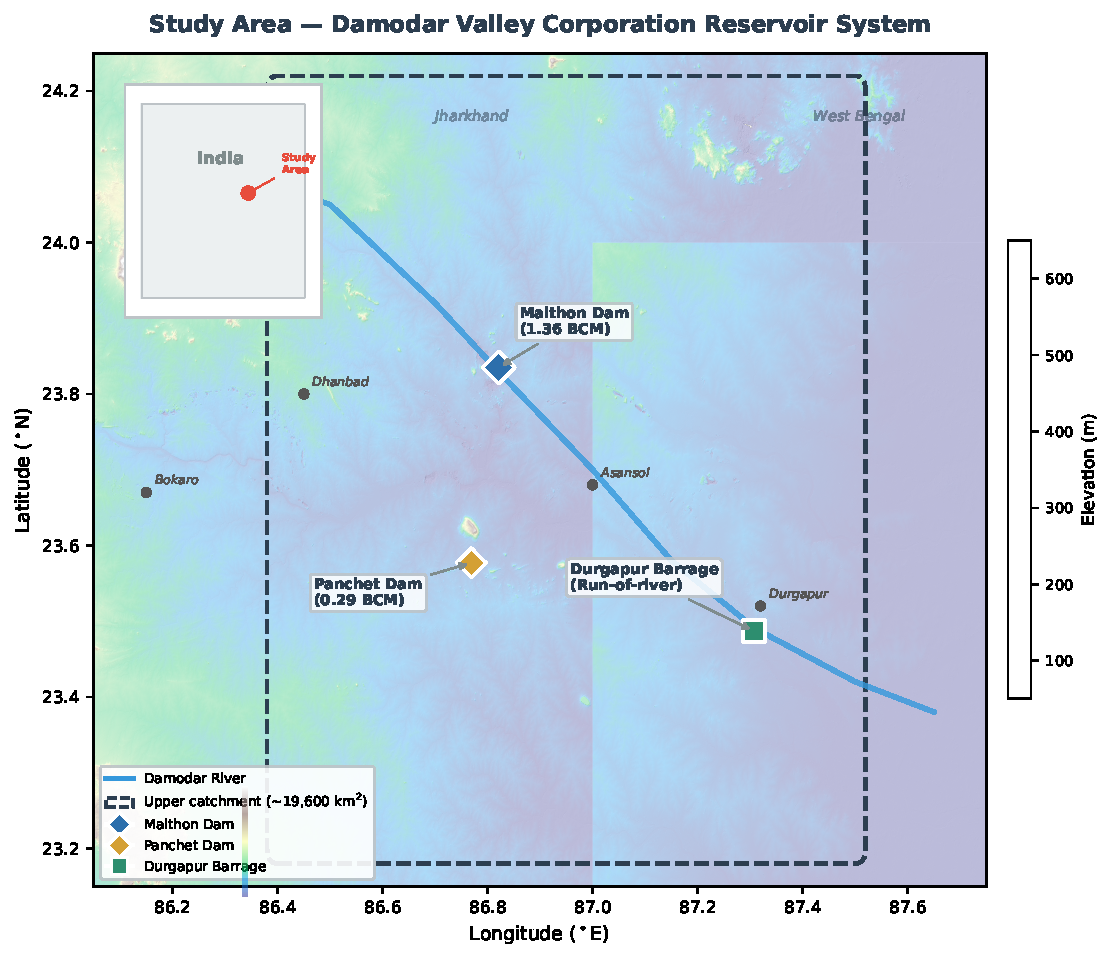
\includegraphics[width=\linewidth]{Fig1_study_area}
  \caption{\textbf{Study area map.} (a) Location of the Damodar Valley
    Corporation (DVC) reservoir cascade in Jharkhand and West Bengal, eastern
    India, overlaid on a MODIS false-colour composite. (b) Sentinel-1 derived
    maximum water extent for Maithon Dam and Durgapur Barrage (2017--2024)
    overlaid on the ALOS AW3D30 DEM hillshade. Panchet Dam is shown as a
    reference structure but was excluded from analysis (see Supplementary
    Note S1). The Damodar catchment boundary (HydroBASINS Level 8) is shown
    in white. Inset: India map showing Jharkhand state.}
  \label{fig:study_area}
\end{figure}

\begin{figure}[htbp]
  \centering
  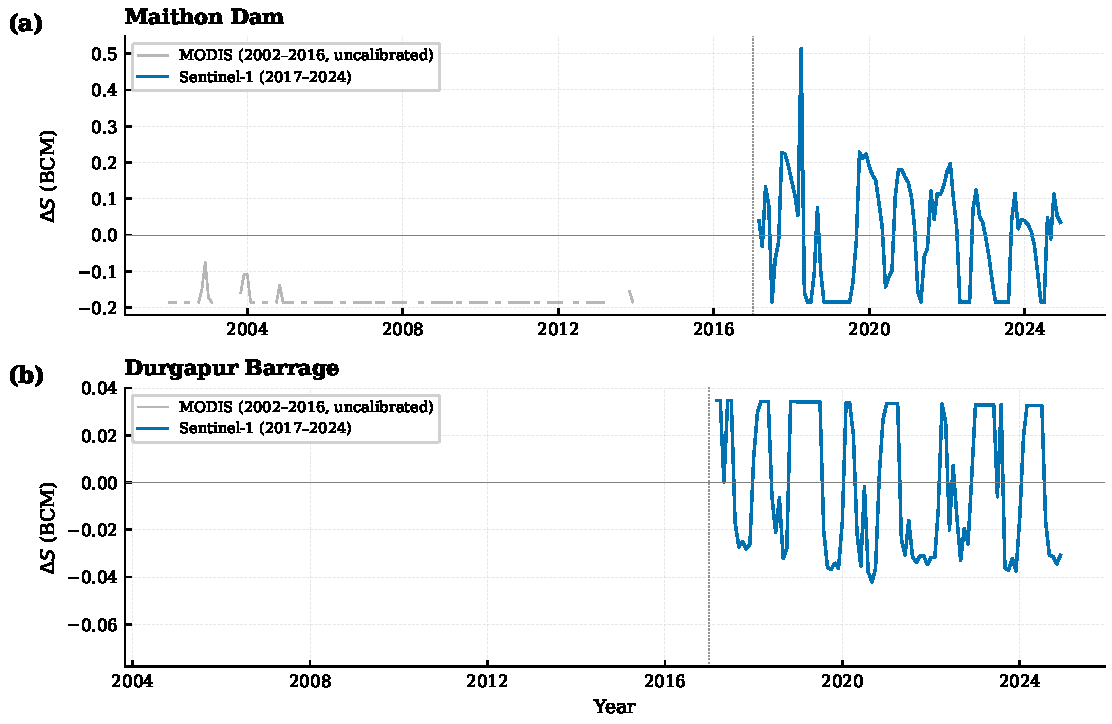
\includegraphics[width=\linewidth]{Fig3_storage_timeseries}
  \caption{\textbf{Reconstructed storage anomaly timeseries 2017--2024.}
    Monthly $\Delta S_{\mathrm{obs}}$ (BCM) for Maithon Dam (blue) and Durgapur
    Barrage (orange), computed relative to the 2017--2023 monthly mean baseline.
    Shaded band indicates $\pm 15$\,\% volumetric uncertainty from the AV curve.
    The Rabi drawdown signature at Durgapur (October--March, orange trough) and
    the 2018 anomalous fill event at Maithon (blue peak, $+0.51\,\mathrm{BCM}$
    above baseline) are labelled.}
  \label{fig:storage_ts}
\end{figure}

\begin{figure}[htbp]
  \centering
  \begin{minipage}[b]{0.48\linewidth}
    \centering
    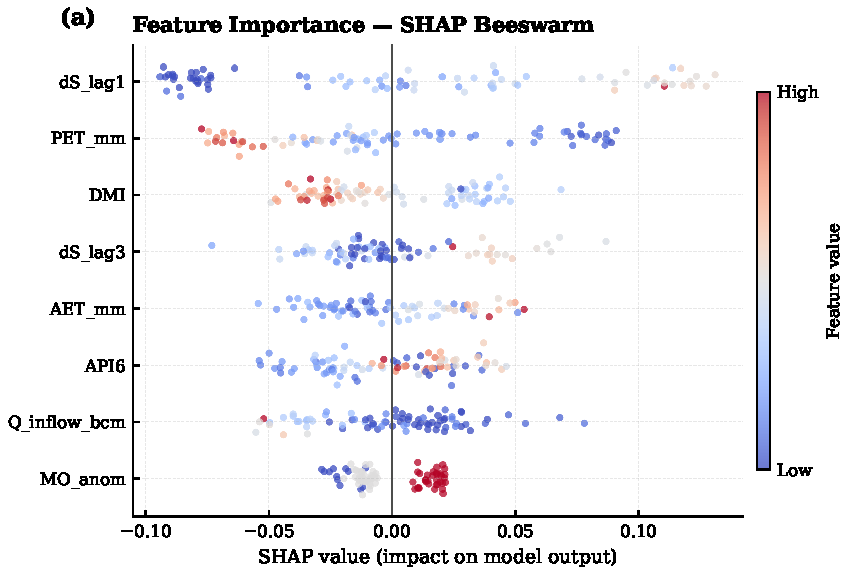
\includegraphics[width=\linewidth]{Fig4a_SHAP_beeswarm}\\
    {\small (a) SHAP beeswarm plot}
  \end{minipage}\hfill
  \begin{minipage}[b]{0.48\linewidth}
    \centering
    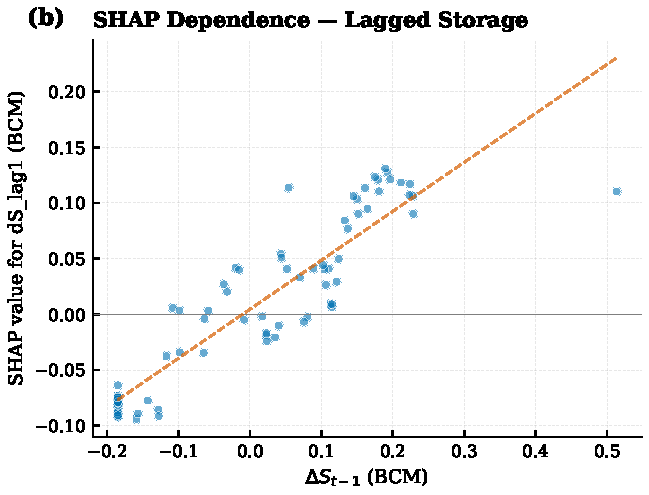
\includegraphics[width=\linewidth]{Fig4b_SHAP_dependence_top}\\
    {\small (b) SHAP dependence: dS\_lag1}
  \end{minipage}
  \caption{\textbf{SHAP feature attribution from the XGBoost climate model.}
    (a) Beeswarm plot showing mean absolute SHAP values ($n = 48$ valid-lag
    rows). Each dot represents one prediction; colour encodes feature value
    (blue\,=\,low, red\,=\,high). Lagged storage anomaly $\Delta S_{\mathrm{lag1}}$
    is the dominant feature (mean $|\mathrm{SHAP}| = 0.064\,\mathrm{BCM}$),
    followed by PET (0.043) and DMI (0.027). (b) SHAP dependence plot for the
    top feature $\Delta S_{\mathrm{lag1}}$, coloured by PET interaction.
    The positive SHAP--feature correlation confirms that high prior-month
    storage predicts higher current storage, consistent with reservoir
    operational persistence.}
  \label{fig:shap}
\end{figure}

\begin{figure}[htbp]
  \centering
  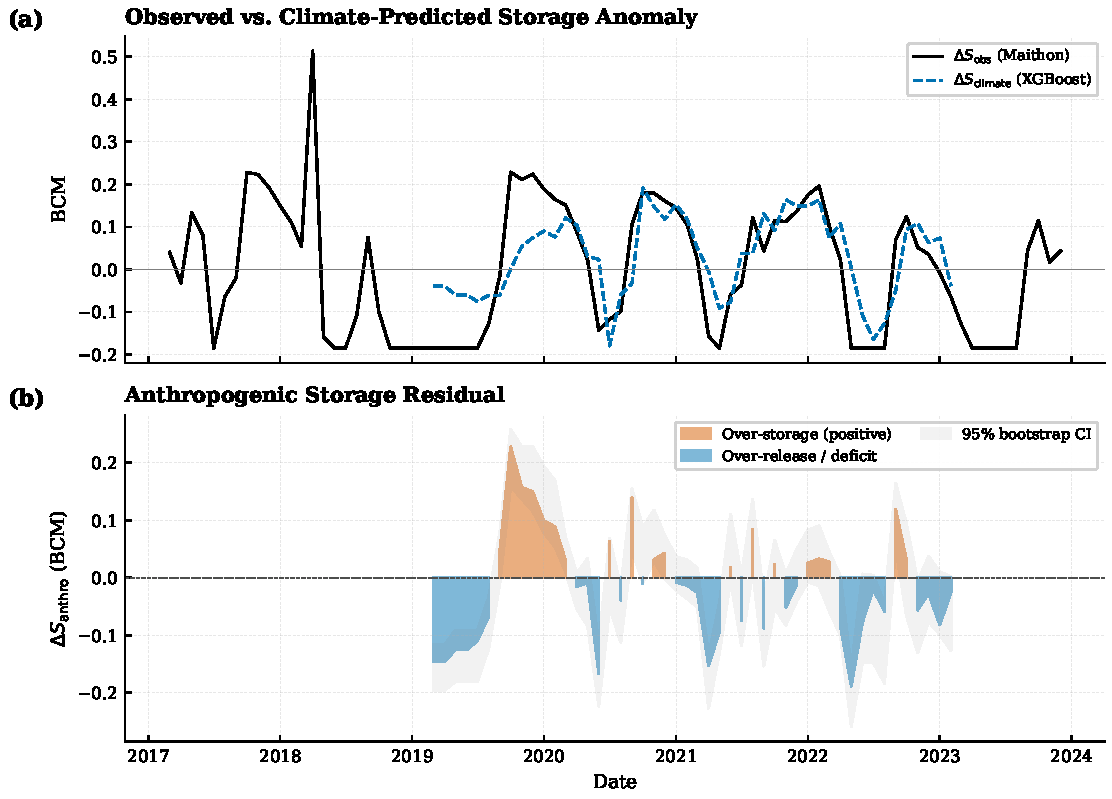
\includegraphics[width=\linewidth]{Fig9_anthro_timeseries}
  \caption{\textbf{Anthropogenic storage anomaly $\dSanthro$ timeseries.}
    Monthly $\dSanthro = \dSobs - \dSclim$ for Maithon Dam (2017--2024).
    Red fill: DRAWDOWN state ($\dSanthro < 0$); blue fill: FILL/NORMAL state.
    HMM state assignments shown on the lower axis (orange\,=\,DRAWDOWN, 25\,\%
    of months; grey\,=\,NORMAL, 75\,\%). Bootstrap 95\,\% CI shown as
    grey shading ($\pm 0.051\,\mathrm{BCM}$).}
  \label{fig:anthro_ts}
\end{figure}

\begin{figure}[htbp]
  \centering
  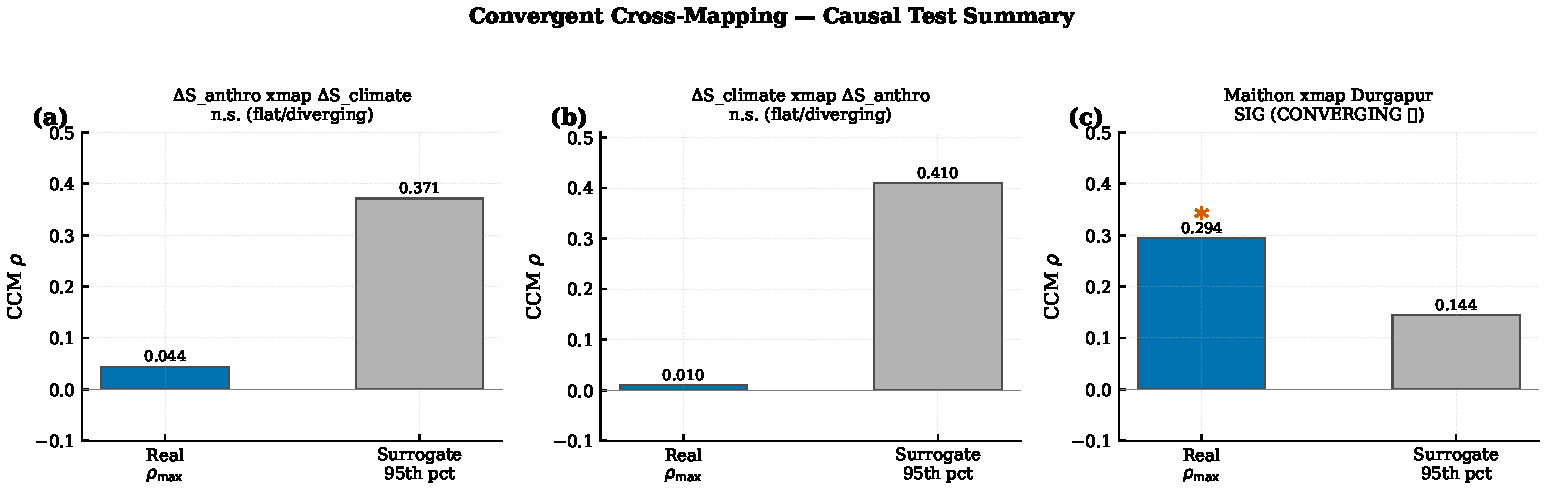
\includegraphics[width=0.8\linewidth]{Fig6c_CCM_convergence}
  \caption{\textbf{Convergent cross-mapping (CCM) results.}
    Cross-map skill $\varrho$ as a function of library size $L$ for Maithon
    $\xrightarrow{\text{xmap}}$ Durgapur (black solid line). Dashed red line
    shows the 95th percentile of 999 phase-randomised surrogates
    ($\text{surr}_{95} = 0.144$). The increasing $\varrho$ with library size
    (convergence slope $= +0.0042$) is the diagnostic signature of genuine
    causal influence (Sugihara et al., 2012). The two null checks ($\dSanthro
    \xmap \dSclim$, blue; $\dSclim \xmap \dSanthro$, green) remain well below
    their respective surrogate thresholds, confirming causal independence of
    the anthropogenic residual from climate predictors.}
  \label{fig:ccm}
\end{figure}

\begin{figure}[htbp]
  \centering
  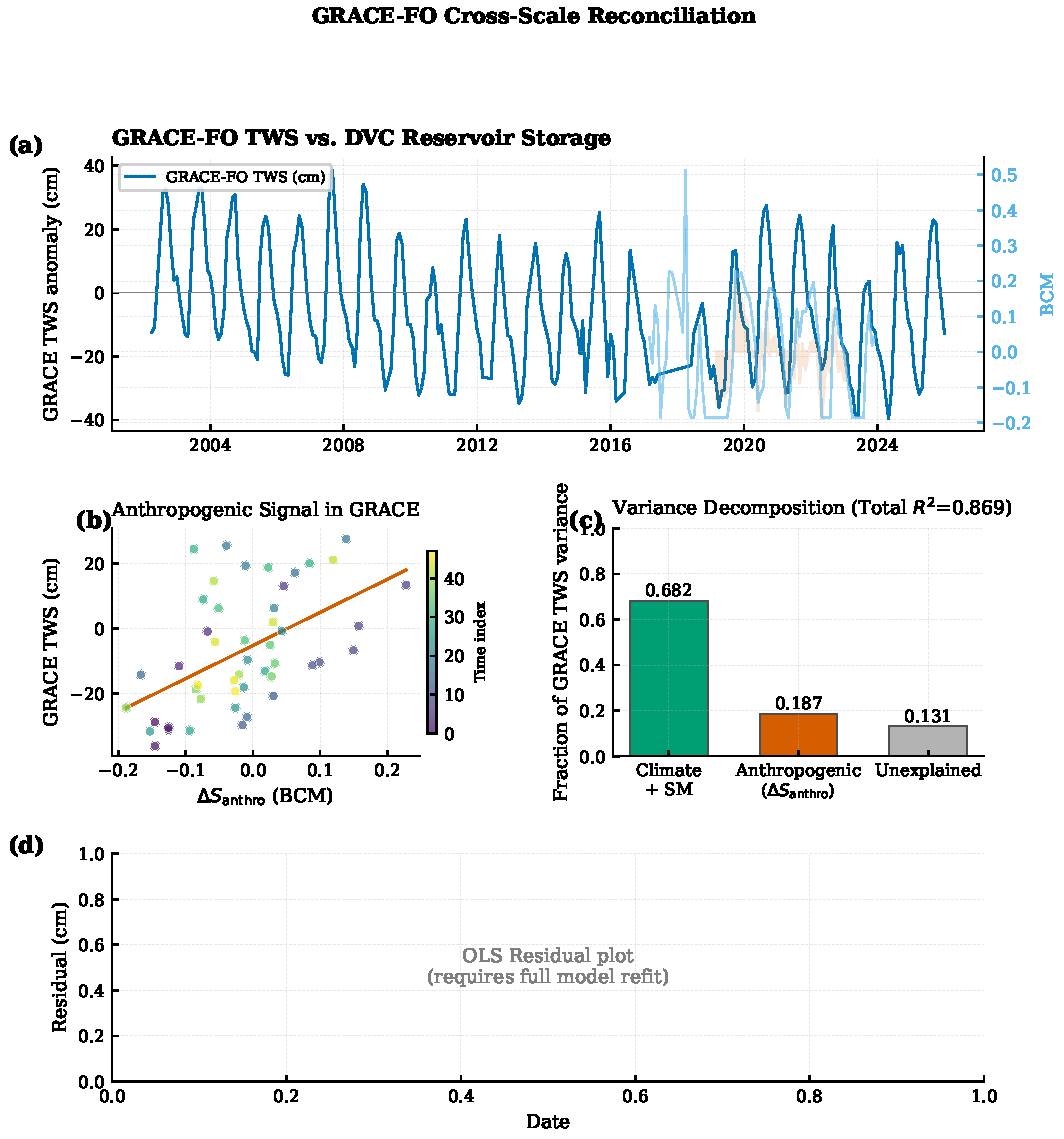
\includegraphics[width=\linewidth]{Fig9_GRACE_reconciliation}
  \caption{\textbf{GRACE-FO cross-scale reconciliation.}
    (a) Observed GRACE-FO TWS anomaly (grey) vs.\ partial OLS model fit
    (red; $R^2 = 0.869$) over the 48-month overlap period. (b) Partial
    regression coefficient $\beta_2$ for $\dSanthro$ with 95\,\% HAC-corrected
    confidence interval ($[+2.13,\,+5.55]$\,cm\,BCM$^{-1}$). The theoretical
    basin sensitivity of $4.28$\,cm\,BCM$^{-1}$ (dashed red line) falls within
    the confidence interval, providing independent physical confirmation of the
    regression result.}
  \label{fig:grace}
\end{figure}

\begin{figure}[htbp]
  \centering
  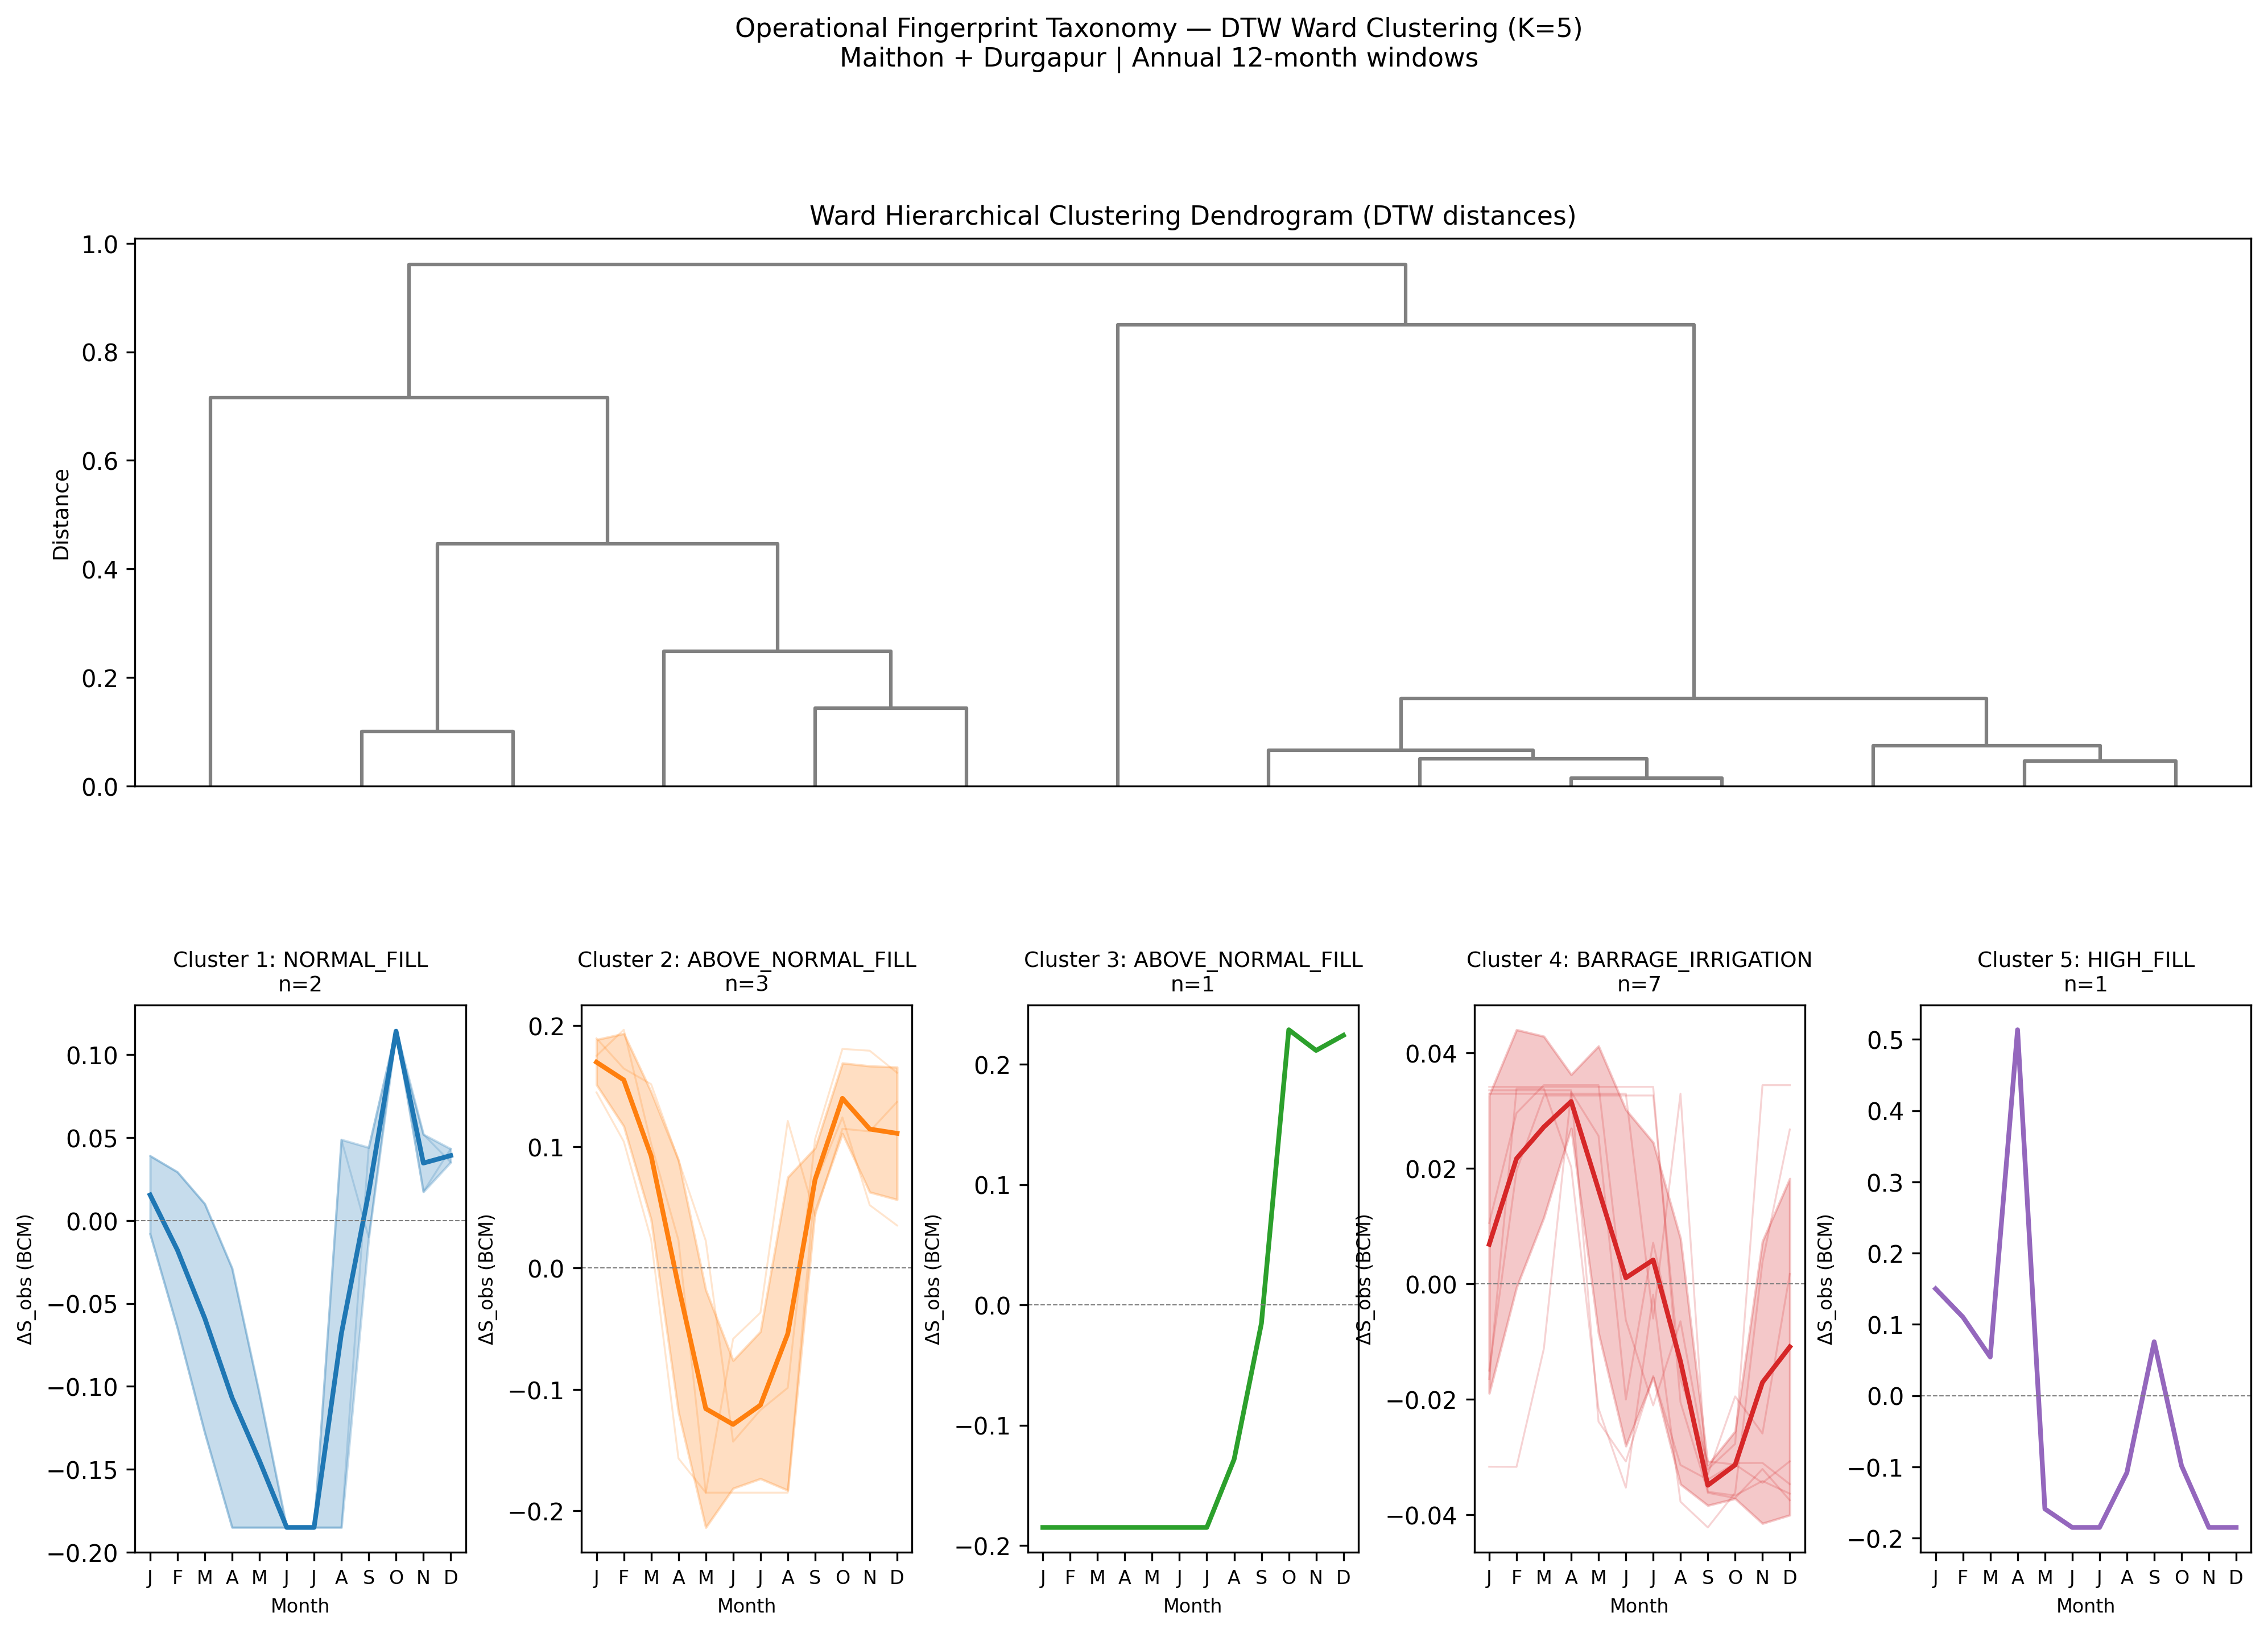
\includegraphics[width=\linewidth]{Fig8_taxonomy}
  \caption{\textbf{Operational fingerprint taxonomy.}
    DTW Ward hierarchical clustering of annual $\Delta S_{\mathrm{obs}}$ cycles
    (2018--2024) for Maithon Dam and Durgapur Barrage, $K = 3$.
    Silhouette score\,=\,0.49. Three operational archetypes are identified:
    Cluster A (Durgapur, all 7 years) --- invariant Rabi irrigation cycle with
    April storage peak and September trough; Cluster B (Maithon 2018) ---
    anomalous high-fill event ($+0.51\,\mathrm{BCM}$ above baseline);
    Cluster C (Maithon 2019--2024) --- standard fill--drawdown cycle with
    declining peak fill fraction over the study period.}
  \label{fig:taxonomy}
\end{figure}

%% =============================================================================
%% SUPPLEMENTARY NOTE S1 — PANCHET EXCLUSION
%% =============================================================================
\clearpage
\section*{Supplementary Note S1: Panchet Dam Exclusion Diagnosis}

The original GEE extraction bounding box for Panchet Dam
($[86.72^\circ,\,23.50^\circ,\,87.05^\circ,\,23.72^\circ]$\,E/N)
inadvertently captured approximately 340\,km$^2$ of the Damodar River
floodplain and sections of the DVC primary canal network south of the dam.
This produced a bimodal water area distribution: 40 records at the expected
40--80\,km$^2$ range (actual reservoir) and 54 records at 140--370\,km$^2$
(canal/floodplain contamination), the latter concentrated in the dry season
when the canal network is flooded for Rabi irrigation delivery. Since the
contamination preferentially affects the seasons most relevant to operational
attribution (pre-monsoon drawdown and post-monsoon conservation), no subset of
the Panchet record is reliable for the purposes of this analysis. The GEE
script has been updated with a corrected tight bounding box
($[86.72^\circ,\,23.52^\circ,\,86.95^\circ,\,23.68^\circ]$); re-running
this extraction is a clear priority for future work to complete the
three-reservoir cascade analysis.

\end{document}
